
\documentclass[conference]{IEEEtran}
% If the IEEEtran.cls has not been installed into the LaTeX system files, 
% manually specify the path to it: e.g.,
% \documentclass[conference]{../sty/IEEEtran} 

\usepackage{graphicx,times,graphicx,amsmath,subfigure} % Add all your packages here

% correct bad hyphenation here
\hyphenation{op-tical net-works semi-conduc-tor IEEEtran}

\IEEEoverridecommandlockouts	% to create the author's affliation portion
				% using \thanks
				
\textwidth 178mm   	% <------ These are the adjustments we made 10/18/2005
\textheight 239mm	% You may or may not need to adjust these numbes again
\oddsidemargin -7mm
\evensidemargin -7mm
\topmargin -6mm 
\columnsep 5mm

\begin{document}


% paper title: Must keep \ \\ \LARGE\bf in it to leave enough margin.
\title{\ \\ \LARGE\bf Distributed Neural Network Training\thanks{Wojciech Dziwulski is with the
Department of Electrical and Computer Engineering,National University of Singapore, 4 Enginnering Drive 3, Sinagpore
(phone:65-9446-7274; email: wojciech.dziwulski@gmail.com).}
}

\author{\textbf{Wojciech Dziwulski} \\ National University of Singapore, University of Oxford}
% avoiding spaces at the end of the author lines is not a problem with
% conference papers because we don't use \thanks or \IEEEmembership
% use only for invited papers
%\specialpapernotice{(Invited Paper)}

% make the title area
\maketitle

\begin{abstract}
This work proposes a novel method of distributing CNN training and processing between several computational units. Our approach utilises the Alternating Direction Method of Multipliers (ADMM) optimization. It minimizes the loss function similarly to the augmented Lagrangian method, but breaks down the optimized variable into two "dual" ones whose minimization is sequential. This allows for cutting down the communication overhead and hence makes the overall method much more memory efficient.

The algorithm is validated, and its performance is evaluated, using the CIFAR10 and MNIST datasets. 
It is proven that the novel setup is able to accommodate a much larger batch size (by factor of 2). This is of large importance because it prospectively allows for training of much deeper network topologies with an architecture distributed between several computational units. The classification accuracy achieved by the dual setup is found to be within the 6\% (CIFAR10) and 0.5\% (MNIST) bound lower than the one achieved by a singular, traditional architecture. Prospectively, this allows for training much deeper network topologies in an architecture distributed between several computational units.
\end{abstract}

% no key words

\section{Introduction}

Understanding data was universally humanity's greatest feat and the need for it is even more compelling nowadays, when the size of datasets is becoming unimaginable. Novel machine learning methods have made great advancements in inference and classification tasks, but the hunger for more robust algorithms and setups grows even quicker. A lot of recent progress is owed to an aggressive increase in the available computation power, allowing us to implement setups that were previously simply unfeasible. More power also means more complicated models, and hence the ability to represent complex functions. As we near the technical limits of single computational units though, we have to turn our research efforts to using distributed approaches allowing us to harness an ever increasing number of clock cycles. This paper presents a novel approach to distributing the computation developed by using a convex optimization algorithm known as ADMM, Alternating Direction Method of Multipliers. 

\section{Background}

\subsection{Machine intelligence}

Deep learning is a term describing neural setups consisting of several processing layers, building up hierarchical features automatically, and hence removing the need for hand-designing them. The networks automatically learn the parameters of convolutional filters that should be applied to the raw input images in order to obtain the desired label. As with traditional neural networks, the weights are learned by computing their gradient with respect to the overall classification error, defined as the 2-norm of the predicted and expected image labels. This is done by running two complimentary algorithms - \textbf{forward} (computing the activations) and \textbf{backward} (computing the updated parameters) \textbf{propagation}.

\subsection{ADMM}

ADMM is a convex optimization algorithm - it tries to find a global minimum of a given loss function. It utilizes the traditional Lagrange multipliers method: $	\min_{x} L(x) = f(x) + \boldsymbol{\lambda^T g(x)}$, but breaks it down into two parts, introducing another, "dual", variable $\boldsymbol{y}$. The loss function then becomes: $\min_{x,y} \max_{\lambda} L(x,y) + \lambda^T (x-y) + \beta ||x-y||^2$. Hence one of our objectives is to minimize the difference between the dual variables, in addition to minimizing the overall loss function. We then proceed with the optimization sequentially, first moving ahead the optimization of x with all the other parameters fixed and then turning to the optimization of y.

\section{Previous work}

The two most notable works devoted to the field of distributed neural network training are those by Dean et al [1] and Chilimbi et al [2]. The first work proposes a framework called DistBelief which parallelizes the training within and between the machines as well as two suitable optimization algorithms - Downpour SGD and Sandblaster L-BFGS. Both offer an inherently parallel optimization method through asynchrounous updates of network parameters and distributing their storage. DistBelief provides model parallelism through distributing the responsibility for node parameter computation between different machines. The node parameters are stored centrally though, on a dedicated parameter server.
The second paper proposes a similar approach, where the parameter and computation servers are disjoint, but where the parameter updates are carried in an asynchronous, lock-free fashion. The model is partitioned vertically, with the convolutional layers separate from the fully connected ones. The forward and back propagation are executed on concurrent threads serving different images. Interestingly, even though this introduces races and usage of not-updated parameter values the overall setup does converge which nicely demonstrates neural nets' resilience to such noise. The approach extends to even 120 machines and trains the networks to an unprecedented accuracy on the MNIST dataset.

\section{ADMM and Deep Learning}

The idea above nicely extends to deep learning. Let's start with breaking down our deep neural network into two parts, duplicating one of the convolutional layers so as to be included in both of the resulting networks. The dual variables x and y will then correspond to the activations of the duplicated layers. Hence the overall optimization is going to consist of two sequential parts: 1) minimizing the difference between the layer activations, 2) minimizing the difference between the predicted and actual image labels.

\section{Experimental setup}

Based on the idea above, a deep neural setup loosely based on CaffeNet was produced and broken down in the fashion shown in figure \ref{net12separate}.

\begin{figure}[htp]
	\centerline{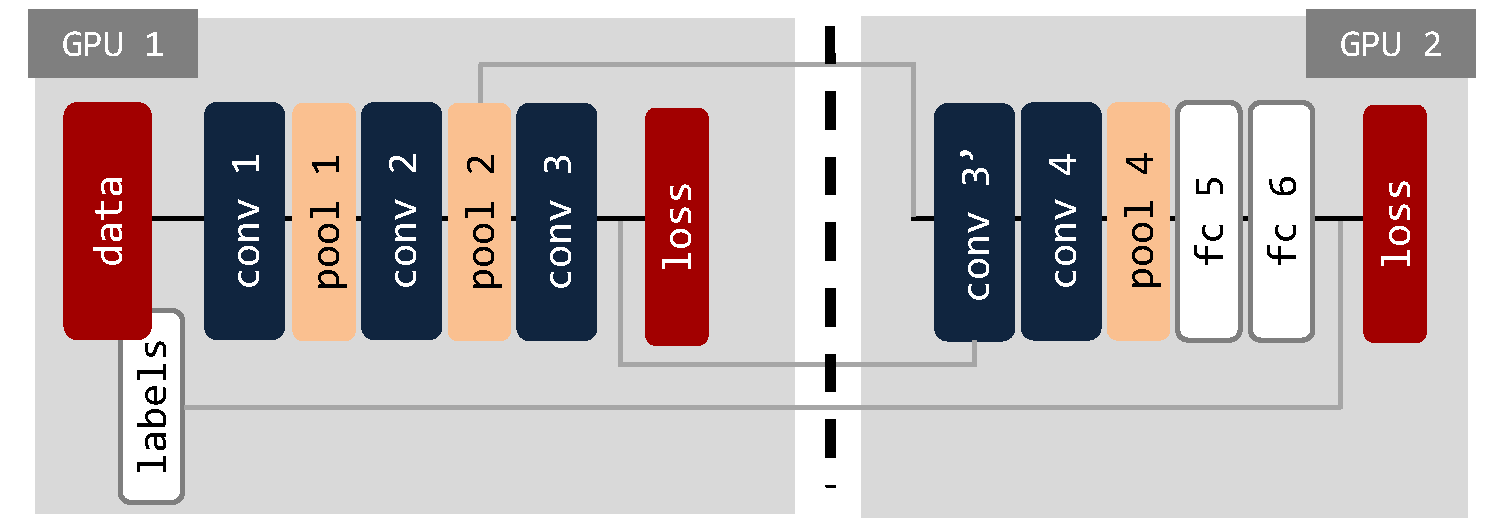
\includegraphics[width=3.35in]{net12separate}}
	\caption{The dual network deep setup.}
	\label{net12separate}
\end{figure}

The setup was implemented and tested using Caffe deep learning framework. The network parameters were stored on the same server, but managed separately and automatically by Caffe. The communication between the two networks was kept to minimum. The parameters that were mutually necessary for computation were the output of layer pool 2, which served as an input to the other part of the network, and the output of layer conv3' (the dual layer), which was necessary to compute the loss function for the first network.

Based on the above considerations the algorithm was finalized as:
\begin{figure}[htp]
	\centerline{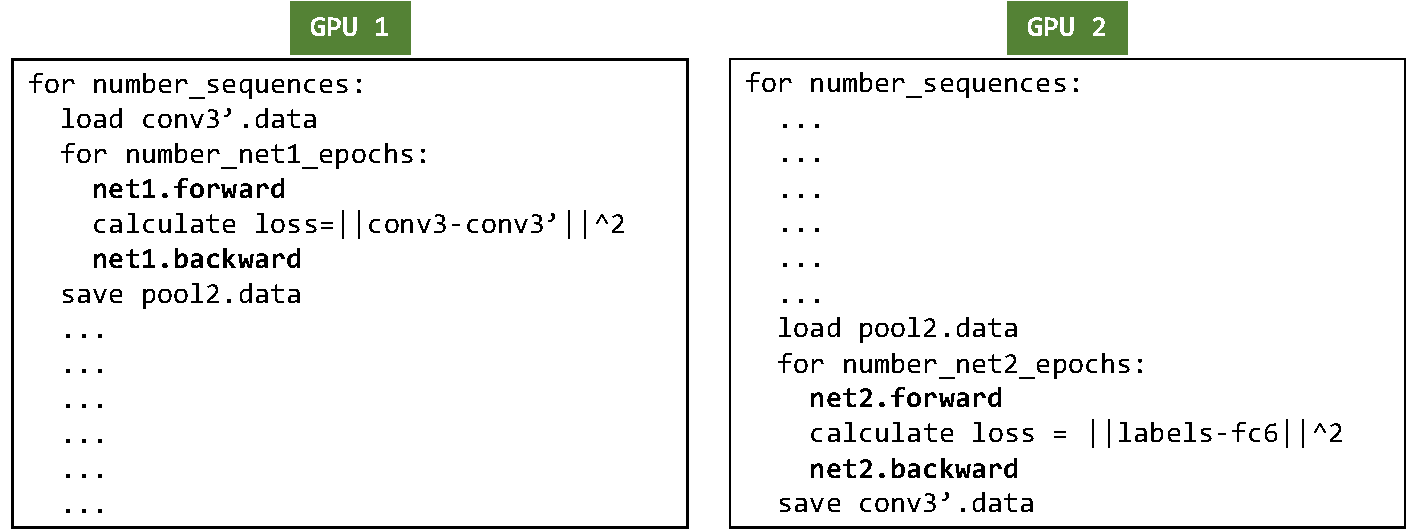
\includegraphics[width=3.35in]{algocode_revisited}}
\end{figure}

\section{Results}

\begin{figure}[htp]
	\centerline{\includegraphics[width=3.35in]{final_2.png}}
	\caption{The final loss function curves.}
	\label{final_2}
\end{figure}

The setup above was tested using the cifar10 and MNIST datasets. The results can be measured against several performance metrics: 1) classification accuracy, 2) loss function value 3) training time 4) maximum batch size, 5) size of the model trained on each machine. Accordingly:

\begin{enumerate}
	\item The classification accuracy achieved after convergence of the networks was within a 6\% bound from the traditional setup in case of cifar10 dataset over three distinct trials. In MNIST, the accuracy was bound by 0.5\%.
	\item As seen in the figure \ref{final_2}, the loss function exhibited very similar behaviour and convergence compared in both single and dual network setups. The characteristic step pattern can be observed in the figure, corresponding to the sequential optimization.
	\item The training time was much larger in case of the dual training, by a factor of around 4, depending on the trial. This is to be expected as the hard drive network communication is far from optimal. This can be easily improved, though, and was not one of the project objectives.
	\item The maximum batch size that could have been fitted in the setup was increased by a factor of 2.
	\item The size of the models individually trained on the GPUs was decreased as well confirming that the dual setup is much more memory efficient. Is is thus proved to be able to train much deeper models, and hence more complicated functions.
\end{enumerate}

\section{Conclusions}

The results above clearly prove the usefulness of the ADMM Deep Learning Distributed approach. It allows for a much more memory-efficient use of the available computational units, hence also permitting to train bigger networks and learning more complicated functions underlying the complex datasets.

The future implementations of the setup should break it down further between more computational units.

                                      
\begin{thebibliography}{1}
	
\bibitem{dean2012large}
J.~Dean, G.~Corrado, R.~Monga, K.~Chen, M.~Devin, M.~Mao, A.~Senior, P.~Tucker,
K.~Yang, Q.~V. Le, et~al.
\newblock Large scale distributed deep networks.
\newblock In {\em Advances in neural information processing systems}, pages
1223--1231, 2012.
\bibitem{chilimbi2014project}
T.~Chilimbi, Y.~Suzue, J.~Apacible, and K.~Kalyanaraman.
\newblock Project adam: Building an efficient and scalable deep learning
training system.
\newblock In {\em 11th USENIX Symposium on Operating Systems Design and
	Implementation (OSDI 14)}, pages 571--582, 2014.



\end{thebibliography}

% that's all folks
\end{document}
